\section{Příklad 5}
% Jako parametr zadejte skupinu (A-H)
\patyZadani{E}

\begin{figure}[b]
    \centering
    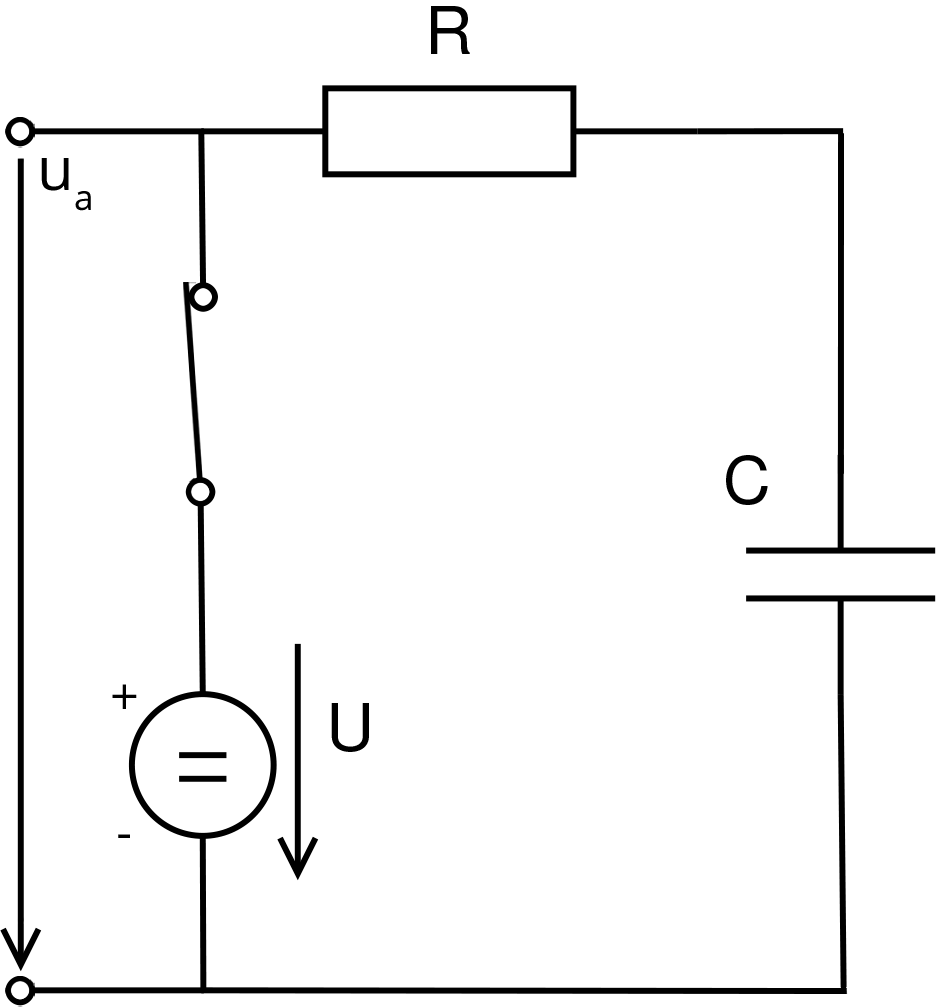
\includegraphics[width=5cm]{diagrams/Diagram13.png}
    \caption{Situace po sepnutí spínače s vyznačeným napětím $u_a$.}
    \label{fig:circ-5-1}
\end{figure}
Za předpokladu, že je spínač a napěťový zdroj ideální, dojde při sepnutí v čase $t = \SI{0}{\second}$ ke skokovému vzrůstu napětí $u_a$ (viz obrázek \ref{fig:circ-5-1}) z 0 V na 40 V. Celým sériovým obvodem prochází stejný proud $i(t)$, pro napětí na rezistoru tak platí:
\[ u_R = R i(t) = 40 i(t) \]
Z druhého Kirchhoffova zákona pak $u_a$ platí:
\[ u_R(t) + u_C(t) - u_1(t) = 0  \]
Protože $u_a$ je od okamžiku $t = 0$ drženo na svorkovém napětí zdroje, můžeme tak zapsat:
\[ u_R(t) + u_C(t) = U \]
Pro proud procházející kondenzátorem, a tedy celým obvodem, platí:
\[
    i_C(t) = i(t) = C\frac{du_C(t)}{dt} = C u_C'(t) = 30 u_C'(t)
\]
Počáteční podmínkou je ze zadání $u_C(0) = 11$. Ze zjištěných vztahů můžeme vytvořit diferenciální rovnici 1. řádu:
\begin{equation} \label{eq:differential}
    40\cdot 30 u_C'(t) + u_C(t) = 40
\end{equation}
Očekávané řešení takovéto rovnice má tvar:
\[
    u_C(t) = f(t) e^{\lambda t}
\]
Sestavíme charakteristickou rovnici, ze které zjistíme konstantu $\lambda$:
\begin{gather*}
    40\cdot 30\lambda + 1 = 0 \\
    \lambda = -\frac{1}{1200}
\end{gather*}
Očekávaným řešením tak je
\begin{equation} \label{eq:exp-solution}
    u_C(t) = f(t) e^{\displaystyle \left(\frac{-t}{1200}\right)}
\end{equation}
jeho derivací pak je
\begin{equation} \label{eq:exp-solution-derived}
    u_C'(t) = f'(t) e^{\frac{-t}{1200}} - \frac{1}{1200} f(t) e^{\frac{-t}{1200}} = \frac{1200 f'(t) e^{\frac{-t}{1200}} - f(t) e^{\frac{-t}{1200}}}{1200}
\end{equation}
Pro zjištění neznámé funkce $f(t)$ dosadíme \eqref{eq:exp-solution} a \eqref{eq:exp-solution-derived} do zadání \eqref{eq:differential}:
\begin{gather*}
    1200\frac{1200 f'(t) e^{\frac{-t}{1200}} - f(t) e^{\frac{-t}{1200}}}{1200} + f(t) e^{\frac{-t}{1200}} = 40 \\
    1200 f'(t) e^{\frac{-t}{1200}} - f(t) e^{\frac{-t}{1200}} + f(t) e^{\frac{-t}{1200}} = 40 \\
    1200 f'(t) e^{\frac{-t}{1200}} = 40 \\
    f'(t) = \frac{1}{30} e^{\displaystyle \left(\frac{t}{1200}\right)}
\end{gather*}
Zintegrováním obou stran zjistíme předpis funkce $f(t)$:
\begin{gather*}
    \int f'(t) = \int \frac{1}{30} e^{\frac{t}{1200}} \\
    f(t) + c_1 = \frac{1}{30} \int e^{\frac{t}{1200}} \\
    f(t) + c_1 = \frac{1}{30} (1200 e^{\frac{t}{1200}} + c_2) \\
    f(t) = 40  e^{\frac{t}{1200}} + c
\end{gather*}
Zjištěnou funkci $f(t)$ dosadíme do očekávaného řešení \eqref{eq:exp-solution}:
\begin{gather*}
    u_C(t) = \left(40  e^{\displaystyle \left(\frac{t}{1200}\right)} + c\right) \cdot e^{\displaystyle \left(\frac{-t}{1200}\right)} \\
    u_C(t) = 40 + c\cdot e^{\displaystyle \left(\frac{-t}{1200}\right)}
\end{gather*}
Pro zjištění konkrétního řešení dosadíme do zjištěného vztahu počáteční podmínku $u_C(0) = 11$:
\begin{gather*}
    u_C(0) = 40 + c\cdot e^0 = 11 \\
    40 + c = 11 \\
    c = -29
\end{gather*}
Konkrétním řešením pro zadané hodnoty tak získáváme rovnici
\[
    \mathbf{u_C(t) = 40 - 29 \cdot e^{\displaystyle \left(\frac{-t}{1200}\right)}}
\]

Posledním krokem jsou kontrolní zkoušky. První zkontrolujeme, jestli platí počáteční podmínka:
\[
    u_C(0) = 40 - 29 \cdot e^{\displaystyle \left(\frac{0}{1200}\right)} = 40 - 29\cdot e^0 = 40 - 29 = 11
\]
Podmínka platí. Dále zkontrolujeme, jestli zjištěná funkce odpovídá rovnici ze zadání \eqref{eq:differential}:
\begin{gather*}
    1200(40 - 29 e^{\frac{-t}{1200}})' + 40 - 29 e^{\frac{-t}{1200}} = 40 \\
    1200(\frac{29}{1200}  e^{\frac{-t}{1200}}) + 40 - 29 e^{\frac{-t}{1200}} = 40 \\
    29 e^{\frac{-t}{1200}} + 40 - 29 e^{\frac{-t}{1200}} = 40 \\
    40 = 40 \\
    L = P
\end{gather*}
Strany se rovnají, nalezená rovnice tak platí.